\chapter{Ausgewählte Aspekte}

\section{Verwendete Hardware}

\subsection{DHT22}

\begin{figure}[H]
    \begin{center}
        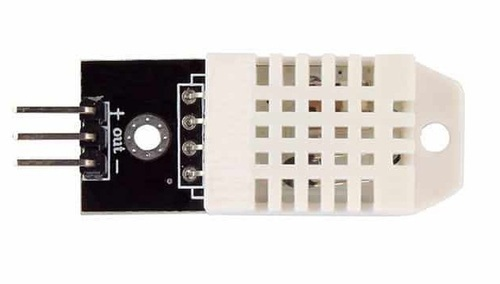
\includegraphics[scale=1]{images/dht22.png}
        \caption{Bild DHT22 \cite{dht22_picture}}
    \end{center}    
\end{figure}



Der DHT22, oder auch AM2302, ist ein digitaler Temperatur und Feuchtigkeissensor, welcher ein digitales Signal der Sensordaten über den Daten-Pin ausgibt. Jedes Exemplar dieses Sensor Modells wurde in einer Kalibriekammer kalibriert. Dieser Kalibrierkoeffizient wird dann im am Bord one time programmable Speicher (OTP Memory \ref{sec:otp}) gespeichert.
\pagebreak

Die Technischen Daten des Sensors sind:
\begin{figure}[H]
    \begin{center}
        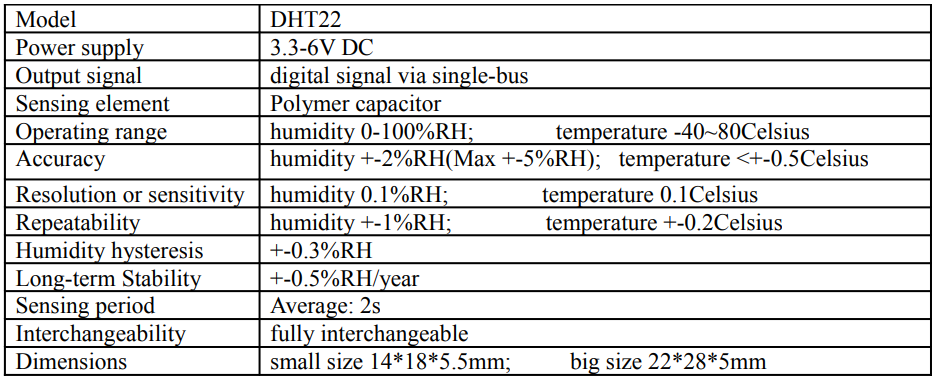
\includegraphics[scale=0.6]{images/dht22_datasheet.png}
        \caption{Daten Dht22 \cite{dht22_datasheet_sparkfun}}
    \end{center}
\end{figure}

Zu den Vorteilen des DHT22 zählen:
\begin{itemize}
    \item Kleiner Formfaktor (15,1mm x 25,1mm x 7,7mm)
    \begin{figure}[H]
        \begin{center}
            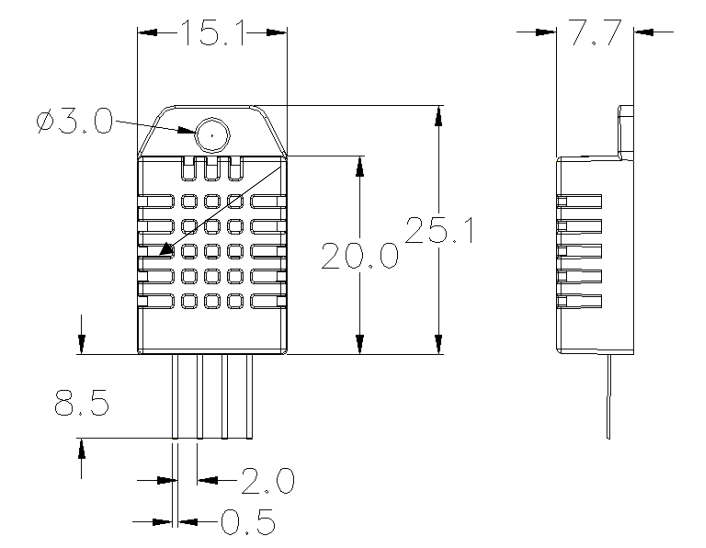
\includegraphics[scale=0.6]{images/dht22_formfaktor.png}
            \caption{Formfaktor Dht22 \cite{dht22_datasheet_sparkfun}}
        \end{center}
    \end{figure}
    \item Niedriger Stromverbrauch (3,3-6 Volt)
    \item Lange Übertragunsdistanz (20 Meter)
\end{itemize}

Der Nachteil des Sensors ist:
\begin{itemize}
    \item Wartezeit zwischen neuen Sensordaten (mindestens 2 Sekunden)
\end{itemize}

\subsubsection{OTP Memory}\label{sec:otp}
OTP Speicher ist eine spezielle Form von nicht flüchtigem Speicher, der es genau ein Mal erlaubt auf den Speicher zu schreiben. Wenn der Speicher einmal programmiert ist behält er seine Informationen für immer, auch über Stromverlust.

Beispiele dafür sind:
\begin{itemize}
    \item Boot code
    \item Encryption keys
    \item Konfigurationsparameter für analoge Sensoren
\end{itemize}

\subsection{NodeMCU ESP32}

\begin{figure}[H]
    \begin{center}
        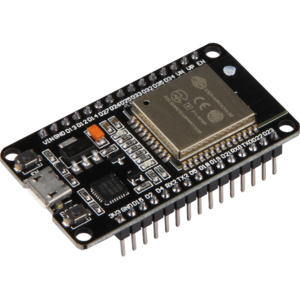
\includegraphics[scale=0.8]{images/NodeMCU-ESP32.png}
        \caption{Bild NodeMCU ESP32 \cite{nodemcu_picture_joy-it}}
    \end{center}
\end{figure}

Das NodeMCU ESP32 ist ein prototyping Board. Die wichtigste Komponente dieses ESPs ist das ESP-WROOM-32 \ref{sec:esp-wroom-32}, es stell das Gehirn dieses Mikrocontrollers dar.

\subsubsection{ESP-WROOM-32}\label{sec:esp-wroom-32}

Das ESP-WROOM-32 ist ein generisches MCU Modul mit integriertem Wi-Fi, Bluetooth und Bluetooth low energy. So ermöglicht einem dieses Modul sich beispielsweise mit Wlan-Router oder einem Handy zu verbinden. Weiters ist es durch den niedrigen Schlafstrom von 5 µA gut für den Bateriebetrieb geeignet.

\begin{figure}[H]
    \begin{center}
        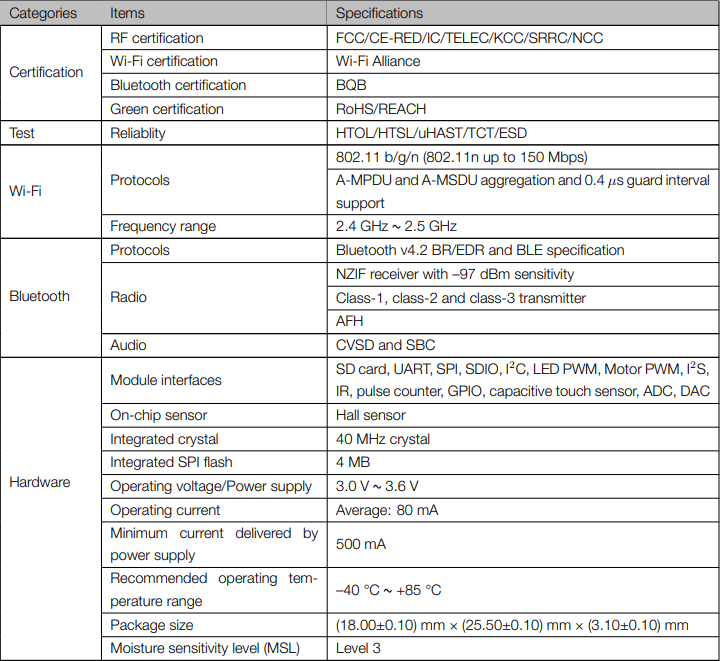
\includegraphics[scale=0.78]{images/esp32-wroom-32.png}
        \caption{ESP32-WROOM-32 Spezifikationen\cite{esp32-wroom-32_secifications}}
    \end{center}
\end{figure}

\section{Over The Air Update (OTA)}\label{sec:ota}

\subsection*{Problemstellung}\label{sec:problem}
Mikrocontroller befinden sich, wenn sie sich in einem laufendem System befinden meist an ungünstigen Orten, an die man nur mit hohem Aufwand gelangt.
Bis jetzt musste man den Computer physisch mit einem Kabel mit dem Mikrocontroller verbinden um neue Firmware auf den Kontroller zu spielen.
OTA ermöglicht es den Mikrocontroller über das Netzwerk mit neuer Firmware zu versorgen, dabei muss der selektierte Microcomputer lediglich mit einem Wlan-Router verbunden sein und ein physisches Kabel wird überflüssig.

\subsection*{Wie OTA funktioniert}
Bei dem OTA-Vorgang wird zu aller erst die Config-Datei, des jeweiligen Mikrocontrollers, ausgelesen. In dierser Datei steht welche Firmware OTA herunterladen soll. Nun sendet der Mikrocontroller eine Anfrage mit dem, in der Config-Datei eingetragen, Namen der Firmware. Diese Anfrage dient dazu den Timestamp, an dem die Firmware das letzte Mal am Server geändert worden ist herauszufinden.\newline
Darauf antwortet der Server mit dem Timestamp.\newline
Nun überprüft der Mikrocontroller den Timestamp der letzten Änderung des Servers mit dem Timestamp der letzten Änderung der Firmware, die gerade installiert ist.\newline

Nun gibt es zwei Szenarien, die eintreten können:

\begin{itemize}
    \item Die Timestamps sind gleich. Das bedeutet, dass der Server und der Mikrocontroller beide die gleiche Firmware besitzen und es besteht kein Grund diese vom Server herunterzuladen.
    \begin{figure}[H]
        \begin{center}
            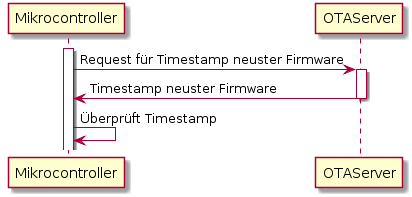
\includegraphics[scale=0.8]{diagrams/ota_sequence_same_timestamp.png}
            \caption{OTA Sequenz Timestamp gleich (Quelle: eigene Darstellung)}
        \end{center}
    \end{figure}
    \newpage
    \item Die Timstamps sind unterschiedlich. Das bedeutet, dass die Firmware am Server geändert wurde und der Mikrocontroller eine ältere Version besitzt.\newline
    Da davon ausgegangen wird, dass der Server immer die beste Version der Firmware bestitz, lädt der Mikrocontroller diese herunter und startet von der soeben heruntergeladenen Firmware neu.
    \begin{figure}[H]
        \begin{center}
            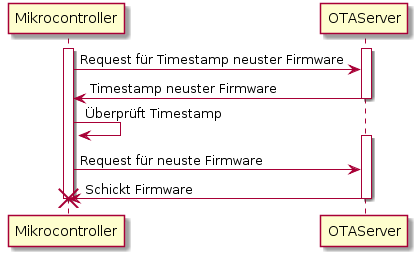
\includegraphics[scale=0.8]{diagrams/ota_sequence_different_timestamp.png}
            \caption{OTA Sequenz Timestamp anders (Quelle: eigene Darstellung)}
        \end{center}
    \end{figure}
\end{itemize}

% TODO: Deployment diagram.
\begin{figure}[H]
    \begin{center}
        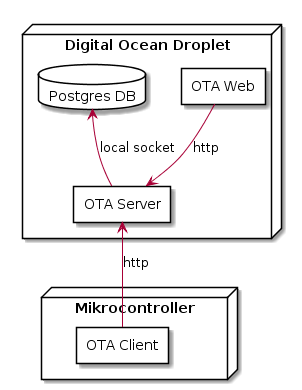
\includegraphics[scale=0.6]{diagrams/ota_deployment.png}
        \caption{OTA Deployment (Quelle: eigene Darstellung)}
    \end{center}
\end{figure}

\subsection{Partition Table}\label{sec:ota-partition-table}
Die Partitionstabelle ist bei OTA mitunter eines der wichtigsten Themen. Würde man diese Tabelle nicht richtig konfigurieren würde das Programm nicht einmal starten. Dazu kommt noch eine erschwerte Fehlersuche, da Errormeldungen bei der Arbeit mit Mikrocontrollern zu wünschen lassen.
Die Standard-Partitionstabelle ist je nach Hersteller anders. Um OTA zu ermöglichen ist es notwendig im Partitionstabelle mindestens eine, ausreichend große, OTA-Partition zu vergeben. Dabei ist es wichtig, dass diese Partition ausreichend Speicher für die gewünschte Firmware hat, da sonst der ganze Vorgang abgebrochen wird.

% TODO: Write about memory diagram
% TODO: Write about partition table diagram

\subsubsection{Übersicht}
Der Flash eines einzelnen ESP32 kann mehrere Apps sowie viele verschiedene Arten von Daten (Kalibrierungsdaten, Dateisysteme, Parameterspeicherung usw.) enthalten. Aus diesem Grund wird eine Partitionstabelle im Flash auf (Standardoffset) 0x8000 geflasht.

Die Länge der Partitionstabelle beträgt 0xC00 Byte (maximal 95 Partitionstabelleneinträge). Nach den Tabellendaten wird eine MD5-Prüfsumme angehängt, mit der die Integrität der Partitionstabelle überprüft wird. Wenn die Partitionstabelle aufgrund eines sicheren Starts signiert ist, wird die Signatur nach der Partitionstabelle angehängt.

Jeder Eintrag in der Partitionstabelle hat einen Namen (Bezeichnung), einen Typ (app, data, ota oder etwas anderes), einen SubType und den Offset im Flash, in dem die Partition geladen wird.

\subsubsection{Custom Partition Tables}
Bei komplexeren Anwendungen reichen die default Partitionstabellen nicht mehr aus und es muss eine angepasste Tabelle erstellt werden, welche aber auch genau auf die Bedürfnisse von gewissen Firmwares zugeschnitten werden kann.

Wenn die Option der Benutzerdefinierte Partitionstabelle ausgewählt wird. Muss manuel eine CSV-Datei erstellt werden, in der dann eine beliebige Anzahl von Partitionen mit folgenden Punkten eingetragen werden können:

\begin{itemize}
    \item Name
    \item SubType
    \item Offset
    \item Size
    \item Flags
\end{itemize}

\begin{figure}[H]
    \begin{center}
        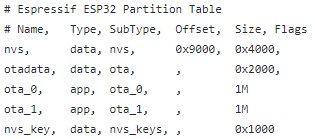
\includegraphics[scale=1]{images/partition_table.png}
        \caption{Beispiel Partitionstabelle (Quelle: eigene Darstellung)}
    \end{center}    
\end{figure}

% TODO: talk about ota partition table diagram

\subsubsection{Name Feld}
Das Namensfeld kann beliebig gewählt werden. Es ist für den Mikrocontroller nicht von Bedeutung. Namen die länger als 16 Zeichen sind werden jedoch abgeschnitten.

\subsubsection{Type Feld}
Das Partitionstypfeld kann als App (0) oder Daten (1) angegeben werden. Oder es kann eine Zahl 0-254 sein (oder als Hex 0x00-0xFE). Die Typen 0x00-0x3F sind für esp-idf-Kernfunktionen reserviert.

Wenn eine Anwendung Daten speichern muss, muss einen benutzerdefinierten Partitionstyp im Bereich 0x40-0xFE hinzugefügt werden.

Der Bootloader ignoriert alle anderen Partitionstypen als App (0) und Daten (1).

\subsubsection{SubType}
Das 8-Bit-SubType-Feld ist spezifisch für einen bestimmten Partitionstyp. Esp-idf gibt derzeit nur die Bedeutung des Subtypfelds für die Partitionstypen "App" und "Daten" an (Stand 09.03.2020).


Wenn der Typ "App" ist, kann das Subtypfeld als Factory (0), ota\_0 (0x10) ... ota\_15 (0x1F) oder test (0x20) angegeben werden.
factory (0) ist die Standard-App-Partition. Der Bootloader führt die Factory-App aus, es sei denn, er sieht eine Partition vom Typ data / ota. In diesem Fall liest er diese Partition, um zu bestimmen, welches OTA-Image gestartet werden soll.
OTA aktualisiert niemals die Factory-Partition.
Wenn Sie die Flash-Nutzung in einem OTA-Projekt beibehalten möchten, können Sie die Factory-Partition entfernen und stattdessen ota\_0 verwenden.
ota\_0 (0x10)\dots ota\_15 (0x1F) sind die OTA-App-Slots. Verwenden Sie dann die OTA-Datenpartition, um zu konfigurieren, welchen App-Slot der Bootloader starten soll. Wenn Sie OTA verwenden, sollte eine Anwendung mindestens zwei OTA-Applikationslots haben (ota\_0 und ota\_1).
test (0x20) ist ein reservierter Subtyp für werkseitige Testverfahren. Es wird als Fallback-Boot-Partition verwendet, wenn keine andere gültige App-Partition gefunden wird. Es ist auch möglich, den Bootloader so zu konfigurieren, dass er bei jedem Start einen GPIO-Eingang liest, und diese Partition zu starten, wenn der GPIO "low" gehalten wird.
Wenn der Typ "data" ist, kann das Subtypfeld als ota (0), phy (1), nvs (2) oder nvs\_keys (4) angegeben werden.
ota (0) ist die OTA-Datenpartition, in der Informationen zur aktuell ausgewählten OTA-Anwendung gespeichert werden. Diese Partition sollte mindestens 0x2000 Bytes groß sein.
phy (1) dient zum Speichern von PHY-Initialisierungsdaten.
In der Standardkonfiguration wird die Phy-Partition nicht verwendet und die PHY-Initialisierungsdaten werden in der App selbst kompiliert. Daher wird diese Partition aus Platzgründen meist aus der Partitionstabelle entfernt.
nvs (2) steht für die NVS-API (Non-Volatile Storage).
NVS wird zum Speichern von PHY-Kalibrierungsdaten pro Gerät verwendet (anders als Initialisierungsdaten).
NVS wird unter anderem zum Speichern von WiFi-Daten verwendet, wenn die Initialisierungsfunktion esp\_wifi\_set\_storage (WIFI\_STORAGE\_FLASH) verwendet wird.
Die NVS-API kann auch für andere Anwendungsdaten verwendet werden.
Es wird dringend empfohlen, eine NVS-Partition von mindestens 0x3000 Byte in Ihr Projekt aufzunehmen, da sonst einige unerwartete Fehler auftreten können.
Wenn Sie die NVS-API zum Speichern vieler Daten verwenden, erhöhen Sie die NVS-Partitionsgröße von den standardmäßig 0x6000 konfigurierten Bytes.
nvs\_keys (4) ist für die NVS-Key-Partition.
Es wird zum Speichern von NVS-encryption-keys verwendet, wenn das NVS Encryption feature aktiviert ist.
Die Größe dieser Partition sollte 4096 Byte betragen (minimale Partitionsgröße).

\subsection{Offset}
Partitionen mit leeren Offsets beginnen nach der vorherigen Partition oder nach der Partitionstabelle bei der ersten Partition.

App-Partitionen müssen an Offsets sein, die auf 0x10000 (64 KB) ausgerichtet sind. Wenn das Offset-Feld leer gelassen wird, richtet gen\_esp32part.py die Partition automatisch aus. Wenn ein nicht ausgerichtetes Offset für eine App-Partition angegeben wird, wird ein Fehler generiert.

Größen und Offsets können als Dezimalzahlen, Hexadezimalzahlen mit dem Präfix 0x oder Größenmultiplikatoren K oder M (1024 und 1024 * 1024 Byte) angegeben werden.

Wenn Sie möchten, dass die Partitionen in der Partitionstabelle mit einem Startoffset (CONFIG\_PARTITION\_TABLE\_OFFSET) der Tabelle selbst funktionieren, lassen Sie das Feld Offset (in der CSV-Datei) für alle Partitionen leer.

\subsubsection{Flags}
Derzeit wird nur ein Flag unterstützt: encrypted. Wenn dieses Feld auf encrypted eingestellt ist, wird diese Partition verschlüsselt, wenn die Flash-Verschlüsselung aktiviert ist.

Partitionen vom App-Typ werden immer verschlüsselt unabhängig ob die Flag gesetzt ist oder nicht.\cite{espressif_partition_tables}

% Todo seite entfernen

\section{Mesh Netzwerk}\label{sec:mesh}
% sequence von http
% sequence von mqtt
% was ist ein mqtt command erklären
% command architektur erlären

\section{NGINX sichern mit letsencrypt}

\section{EspWifiManager Implementation}

\section{Makeconfig}

\section{Die Wichtigkeit von Erase Flash}

\section{Mesh Visualizer}\label{sec:mesh-visualizer}

\section{Libraries}

\subsection{Mqtt}
\subsection{Http}
\subsection{Mesh}
\subsection{Dht22}

\section{Bedienungsanleitung}

\subsection{Übersicht}

\vspace*{50px}
\begin{figure}[H]
    \begin{center}
        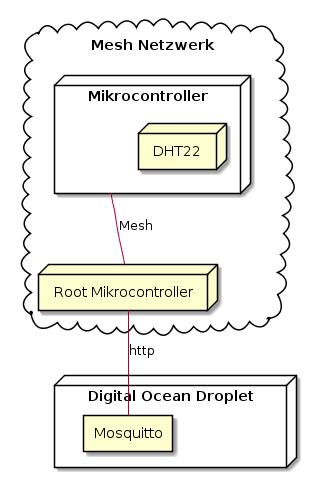
\includegraphics[scale=.5]{diagrams/mqtt_dht22_example_deployment.png}
        \caption{Deployment Diagramm (Quelle: eigene Darstellung)}
    \end{center}    
\end{figure}

In diesem kleinen Beispiel gibt es insgesamt 2 Mikrocontroller. 

\begin{itemize}
    \item Ein \textbf{Mikrocontroller} welcher mit einem DHT22 verbunden ist und regelmäßig die Sensordaten weiterschickt.
    \item Ein \textbf{Root Mikrocontroller} der nur für das weiterleiten der Nachrichten zuständig ist.
\end{itemize}

Der Root Mikrocontroller ist mit einem MQTT Broker (\textbf{Mosquitto}) verbunden.

Der \textbf{Mosquitto} Server läuft auf einer beliebigen \textbf{Host Machine} (Bsp.: Digital Ocean Droplet).

\vspace*{50px}
\begin{figure}[H]
    \begin{center}
        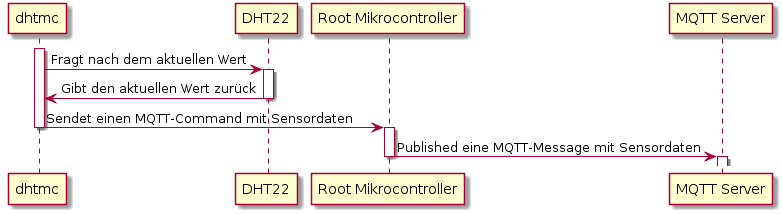
\includegraphics[scale=.5]{diagrams/mqtt_dht22_example_sequence.png}
        \caption{Sequence Diagramm (Quelle: eigene Darstellung)}
        \label{abb:dht22_sequence_diagram}
    \end{center}
\end{figure}
\vspace*{50px}

Die Abbildung \ref{abb:dht22_sequence_diagram} zeigt den Verlauf einer Iteration dieses Beispieles.
Der \textbf{dhtmc} (Der \textbf{Mikrocontroller} des Deployment Diagramms) ließt die aktuellen Werte des DHT22, welche er dann in dem Mesh Netzwerk mittels MQTT Command verschickt.

Wenn der \textbf{Root Mikrocontroller} diesen neuen MQTT Command bekommt schickt er die MQTT Nachricht an den angegebenen \textbf{MQTT Server} weiter.

Es wird davon ausgegangen, dass eine Installation von Nodejs mit einer Version von mindestens \textit{10} vorhanden ist.

Die Installation wird in Kapitel \ref{sec:nodejs} beschrieben.

\subsection{ESP-IDF Setup}

Die folgenden Anweisungen setzen ein Ubuntu-Betriebssystem vorraus. Es wird nicht garantiert, dass dies unter Alternativen wie zum Beispiel dem \textbf{Windows Subsystem for Linux (WSL) \ref{sec:wsl}} funktioniert. 

\subsubsection{Dependencies}

Zu aller erst müssen die Dependencies von ESP-IDF installiert werden. Dafür gibt es den folgenden shell command.

\vspace*{10px}
\begin{verbatim}
    sudo apt-get install git wget flex bison gperf python python-pip 
    python-setuptools cmake ninja-build ccache libffi-dev libssl-dev
\end{verbatim}
\vspace*{10px}

\subsubsection{Libraries}\label{sec:libraries}

Damit man die ESP-IDF Libraries benutzen kann, muss man diese zuerst herunterladen.

\vspace*{10px}
\begin{verbatim}
    mkdir $HOME/esp &&
    cd $HOME/esp &&
    git clone --recursive https://github.com/espressif/esp-idf.git
\end{verbatim}
\vspace*{10px}

Mit den obigen Befehlen erstellt man zuerst einen neuen Ordner im Homeverzeichnis des aktuell eingeloggten Benutzer und wechselt in diesen. 
Anschließend wird das offizielle Repository von ESP-IDF rekursiv gecloned.

Nachdem das Repository erfolgreich gecloned wurde, muss man die Libraries installieren. Dies erfolgt durch folgende Bash Befehle.

\vspace*{10px}
\begin{verbatim}
    cd $HOME/esp/esp-idf &&
    ./install.sh
\end{verbatim}
\vspace*{10px}

Mit diesen Befehlen wird das Arbeitsverzeichnis auf das vorher installierte Repository gesetzt und die \textbf{install.sh} Datei von ESP-IDF ausgeführt.

Dies kann einige Minuten dauern.

\subsubsection{Umgebungsvariablen}

Damit die Toolchain nun verwendet werden kann, müssen noch ein paar Umgebungsvariablen definiert werden. 

\vspace*{10px}
\begin{verbatim}
    export IDF_PATH=$HOME/esp/esp-idf
\end{verbatim}
\vspace*{10px}

Die \textit{IDF\_PATH} Variable gibt den Pfad des Repositories von ESP-IDF an.

\vspace*{10px}
\begin{verbatim}
    . $HOME/esp/esp-idf/export.sh
\end{verbatim}
\vspace*{10px}

Danach müssen noch weitere Umgebungsvariablen von ESP-IDF selbst gesetzt werden, dafür muss man den oben angeführten Befehl ausführen.

Diese Variablen werden nur für die aktuelle Shell-Session gesetzt, deswegen wäre es sinnvoll diese Befehle in die \textbf{.bashrc} Datei im Homeverzeichnis zu schreiben.

\vspace*{10px}
\begin{verbatim}
    export IDF_PATH=$HOME/esp/esp-idf
    . $HOME/esp/esp-idf/export.sh
\end{verbatim}
\vspace*{10px}

Es ist auch möglich eine eigene Funktion dafür zu definieren, wenn man die Toolchain nur bei bedarf benutzen möchte.

\vspace*{10px}
\begin{verbatim}
    function loadEspIdf() {
        export IDF_PATH=$HOME/esp/esp-idf
        . $HOME/esp/esp-idf/export.sh
    }
\end{verbatim}
\vspace*{10px}

Anschließend muss der Terminal neugestartet werden, um die \textbf{.bashrc} Datei ausführen zu können.

\subsubsection{WSL}\label{sec:wsl}

WSL unterstützt bis zum Stand vom \textbf{29.03.2020} das Linux USB Interface nicht. Dies bedeutet, dass für eine fehlerfreie Nutzung der ESP-IDF-Toolchain nicht garantiert wird.

\subsection{Source Code}\label{sec:example-source-code}

Der Source Code der für dieses Beispiel benötigt wird, lebt in dem folgenden Repository.

\vspace*{10px}
\begin{verbatim}
    https://github.com/TimUntersberger/Diplomarbeit
\end{verbatim}
\vspace*{10px}

Für die erfolgreiche Absolvierung des Beispieles ist es notwendig das Repository zu clonen.

\vspace*{10px}
\begin{verbatim}
    git clone https://github.com/TimUntersberger/Diplomarbeit
\end{verbatim}
\vspace*{10px}

Nachdem der Command fertig ist, befinden sich mehrere Unterordner in dem neu erstellten Ordner namens \textit{Diplomarbeit}. Die einzigen relevanten Ordner für das Beispiel sind \textbf{Dht22Example} und \textbf{MeshVisualizer}.

Nach Bedarf können die anderen gelöscht werden.

Die zwei Dateien, welche in Kapitel \ref{sec:mosquitto} beschrieben werden, befinden sich in dem Unterordner \textbf{MeshVisualizer}.

Genauere Anweisungen zu \textbf{MeshVisualizer} befinden sich in dem Kapitel \ref{sec:example-mesh-visualizer}.

Die Struktur und wie der Code von \textbf{Dht22Example} benutzt werden kann, wird in dem Kapitel \ref{sec:code} beschrieben.

\subsection{Mosquitto}\label{sec:mosquitto}

\textbf{mosquitto.conf}
\begin{verbatim}
    listener 1883
    protocol mqtt

    listener 1884
    protocol websockets
\end{verbatim}
\vspace*{10px}

Die \textbf{mosquitto.conf} Datei konfiguriert den Mosquitto Broker so, dass er auf 2 Ports zu hört.

\begin{enumerate}
    \item 1883
    \item 1884
\end{enumerate}

Auf dem Port \textbf{1883} hört ein Websocket Server zu, welcher für die Nutzung von dem \textbf{Mesh Visualizer} \ref{sec:mesh-visualizer} konfiguriert wurde. 

Der Port 1883 ist wie üblich eine MQTT-Schnittstelle.

\textbf{docker-compose.yml}
\begin{verbatim}
    version: '3'
    services:
      mosquitto:
        image: eclipse-mosquitto
        ports:
          - '1883:1883'
          - '1884:1884'
        volumes:
            - ./mosquitto.conf:/mosquitto/config/mosquitto.conf
\end{verbatim}
\vspace*{10px}

Diese \textbf{docker-compose.yml} Datei verwendet die Version 3 von docker-compose. Insgesamt wird nur ein einziger Service benötigt für dieses Beispiel. Der Name des Services ist \textit{mosquitto} und benützt das offizielle Image von eclipse namens \textit{eclipse-mosquitto}.

Wie schon bei der \textbf{mosquitto.conf} Datei erwähnt, benötigt Mosquitto 2 offene Ports. Diese werden hier mit den selben äußeren Ports verbunden.

Die Konfigurationsdatei wird mittels eines Volumen in den Container injected.

In der folgenden Abbildung (\ref{abb:example_mosquitto_start}) ist zu sehen wie man den Mosquitto nun startet.

\begin{figure}[H]
    \begin{center}
        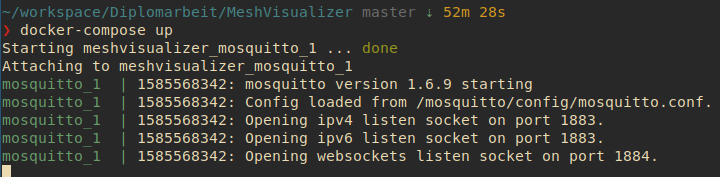
\includegraphics[scale=0.8]{images/example_mosquitto_start.png}
        \caption{Example Mosquitto Start (Quelle: eigene Darstellung)}
        \label{abb:example_mosquitto_start}
    \end{center}
\end{figure}

\subsection{Mesh Visualizer}\label{sec:example-mesh-visualizer}

Nach der erfolgreichen Absolvierung der in Kapitel \ref{sec:example-source-code} beschriebenen Anweisungen befindet sich nun der Unterordner namens \textbf{MeshVisualizer} in dem Ordner Diplomarbeit.

Bevor der \textbf{MeshVisualizer} gestartet werden kann, muss das Arbeitzverzeichnis auf den Pfad des \textbf{MeshVisualizer} Ordners gesetzt werden.

Anschließend ist es notwendig, die Dependencies des Projekts zu installieren.

Dies erfolgt durch den in Abbildung \ref{abb:example_mesh_visualizer_installation_cmd} angeführten Command.

\begin{figure}[H]
    \begin{center}
        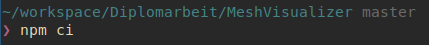
\includegraphics[scale=1]{images/example_mesh_visualizer_installation_cmd.png}
        \caption{Example Mesh Visualizer Installation Command (Quelle: eigene Darstellung)}
        \label{abb:example_mesh_visualizer_installation_cmd}
    \end{center}
\end{figure}

\pagebreak
In der nachstehenden Abbildung (\ref{abb:example_mesh_visualizer_installation_output}) wird das Ergebnis visualisiert.

\begin{figure}[H]
    \begin{center}
        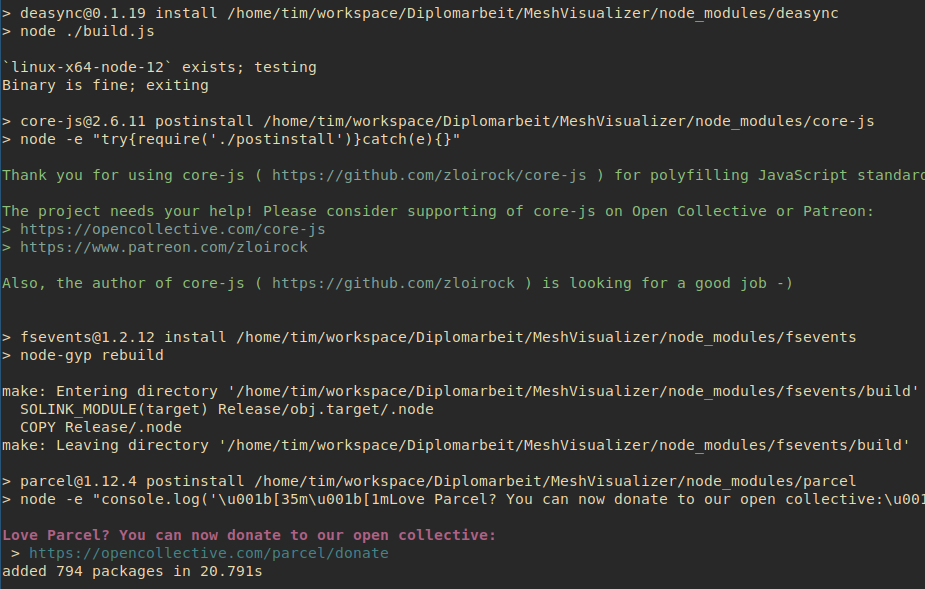
\includegraphics[scale=.6]{images/example_mesh_visualizer_installation_output.png}
        \caption{Example Mesh Visualizer Installation Output(Quelle: eigene Darstellung)}
        \label{abb:example_mesh_visualizer_installation_output}
    \end{center}
\end{figure}

Das starten des Visualizers geschieht wie in der nachstehenden Abbildung (\ref{abb:example_mesh_visualizer_start}).

\begin{figure}[H]
    \begin{center}
        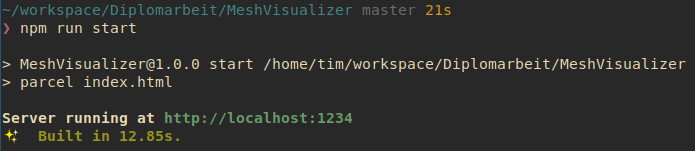
\includegraphics[scale=.6]{images/example_mesh_visualizer_start.png}
        \caption{Example Mesh Visualizer Start (Quelle: eigene Darstellung)}
        \label{abb:example_mesh_visualizer_start}
    \end{center}
\end{figure}

Nachdem der Server auf dem Port \textit{1234} läuft, ist nun die Website, welche in Abbildung \ref{abb:example_mesh_visualizer_website} zu sehen ist, auf der URL \textit{http://localhost:1234/} verfügbar.

\begin{figure}[H]
    \begin{center}
        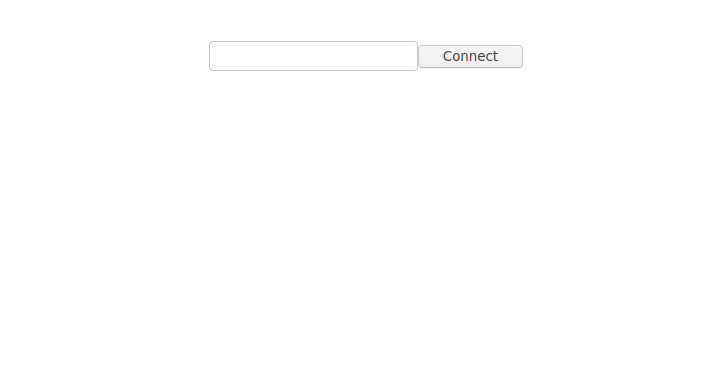
\includegraphics[scale=.3]{images/example_mesh_visualizer_website.png}
        \caption{Example Mesh Visualizer Website (Quelle: eigene Darstellung)}
        \label{abb:example_mesh_visualizer_website}
    \end{center}
\end{figure}

Auf der Website ist momentan nur ein Eingabefeld zusammen mit einem Knopf direkt daneben zu sehen.

Durch das Eingabefeld wird die URL des Mosquittos gesetzt. 
Die Definierung des verwendeten Protokolls darf nicht auser Acht gelassen werden.\newline

Da Javascript im Browser nicht in der Lage ist mit dem MQTT Protokoll zu kommunizieren, muss man sich mit dem vorher definierten Websocket Port (1884) des Brokers verbinden.

Beispiel
\begin{verbatim}
    ws://localhost:1884
\end{verbatim}

Mit dem Drücken des \textit{connect} Knopfs, wird versucht eine Verbindung mit dem Broker herzustellen.

Die Benutzung der Website wird in Kapitel \ref{sec:example-result} genauer erläutert.

\subsection{Partition Table}

\begin{figure}[H]
    \begin{center}
        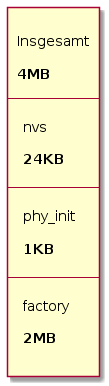
\includegraphics[scale=.6]{diagrams/mqtt_dht22_example_partitions.png}
        \caption{Example Partiton Table (Quelle: eigene Darstellung)}
        \label{abb:example-partitions}
    \end{center}
\end{figure}

Der verwendete Mikrocontroller besitzt insgesamt \textbf{4MB} an Speicher.

Für das Programm sind \textbf{2MB} reserviert, da der default Wert von \textbf{1MB} für dieses Beispiel nicht ausreichend ist. 

Mehr Informationen zu \textit{Partition Tables} sind in Kapitel \ref{sec:ota-partition-table} zu finden.

\subsection{Config}

Die Konfiguration eines ESP-IDF Projekts, wird im Normfall mittels der menuconfig gelöst, wie in Kapitel \ref{sec:esp-idf-toolchain} erwähnt.

\pagebreak

Nachdem öffnen der menuconfig sind die folgenden Optionen abgebildet.

\begin{figure}[H]
    \begin{center}
        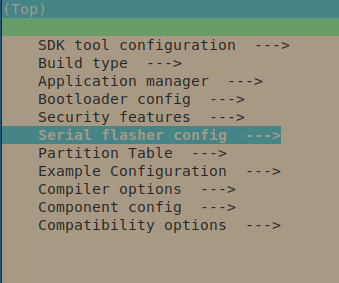
\includegraphics[scale=1]{images/example_config_overview.png}
        \caption{Example Config Übersicht (Quelle: eigene Darstellung)}
        \label{abb:example_config_overview}
    \end{center}
\end{figure}

Die folgenden Optionen werden im Laufe dieses Kapitels berührt:

\begin{enumerate}
    \item Example Configuration (Kapitel \ref{sec:example-example-config})
    \item Serial flasher config (Kapitel \ref{sec:example-serial-flasher-config})
    \item Partition Table (Kapitel \ref{sec:example-partition-table})
\end{enumerate}

Nachdem das Programm fertig konfiguriert ist, kann die menuconfig geschlossen werden.

\pagebreak

\subsubsection{Example Configuration}\label{sec:example-example-config}

In der \textbf{Example Configuration} Option wird das Mesh Netzwerk und der MQTT-Client konfiguriert.

\begin{figure}[H]
    \begin{center}
        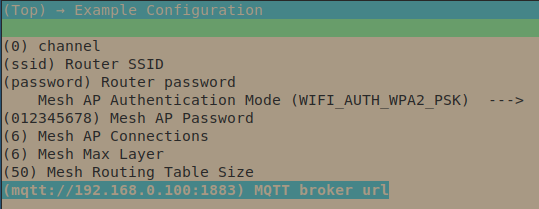
\includegraphics[scale=1]{images/example_config_example_config.png}
        \caption{Example Config Example Configuration (Quelle: eigene Darstellung)}
        \label{abb:example_config_example_config}
    \end{center}
\end{figure}

Folgende Werte müssen angepasst werden:

\begin{itemize}
    \item \textbf{Router SSID} \newline
        Die SSID des WLAN Routers, womit sich der Mikrocontroller verbinden soll.
    \item \textbf{Router password} \newline
        Das Passwort des WLAN Routers, womit sich der Mikrocontroller verbinden soll.
    \item \textbf{Mesh AP Password} \newline
        Das Mesh-Netzwerk interne Passwort. Das Passwort muss mindestens 8 Zeichen lang sein und mindestens eine Zahl beinhalten.
    \item \textbf{MQTT broker url} \newline
        Die URL des MQTT Brokers. Hier ist es wichtig, dass nicht localhost eingegeben wird, da dieses Programm auf dem esp läuft (dies ist am Anfang der Arbeit passiert).\newline
        Das Schema muss der URL in dem Beispiel unten in Abbildung \ref{abb:example_config_example_config} folgen.
\end{itemize}

\pagebreak

\subsubsection{Serial flasher config}\label{sec:example-serial-flasher-config}

In der \textbf{Serial flasher config} Option wird der Serial Flasher konfiguriert.

\begin{figure}[H]
    \begin{center}
        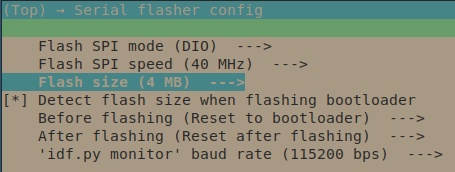
\includegraphics[scale=1]{images/example_config_serial_flasher_config.png}
        \caption{Example Config Serial Flasher Config (Quelle: eigene Darstellung)}
        \label{abb:example_config_serial_flasher_config}
    \end{center}
\end{figure}

Hier muss nur die \textbf{Flash size} angepasst werden. Die Größe hängt von dem jeweiligen Modell des ESPs ab.

\subsubsection{Partition Table}\label{sec:example-partition-table}

In der \textbf{Partition Table} Option wird der verwendete \textit{Partition Table} konfiguriert.

\begin{figure}[H]
    \begin{center}
        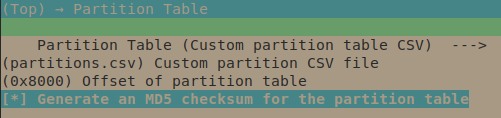
\includegraphics[scale=1]{images/example_config_partition_table.png}
        \caption{Example Config Partition Table (Quelle: eigene Darstellung)}
        \label{abb:example_config_partition_table}
    \end{center}
\end{figure}

In dieser Konfiguration muss der Typ des \textbf{Partition Table} Felds auf \textit{Custom partition table CSV} gesetzt werden.

\subsection{Hardware}
% TODO: write about how to connect the dht22 with the esp
% TODO: write about how to connect the esp with the computer

\subsection{Flashen}

Bevor das Programm auf den ESPs laufen kann, muss es hochgeladen werden.

Das Hochladen bzw. Flashen eines Programms verläuft wie in Kapitel \ref{sec:esp-idf-toolchain} beschrieben.

\subsection{Ergebnis}\label{sec:example-result}
% TODO: Explain Result
\subsubsection{Mesh Visualizer}

\begin{figure}[H]
    \begin{center}
        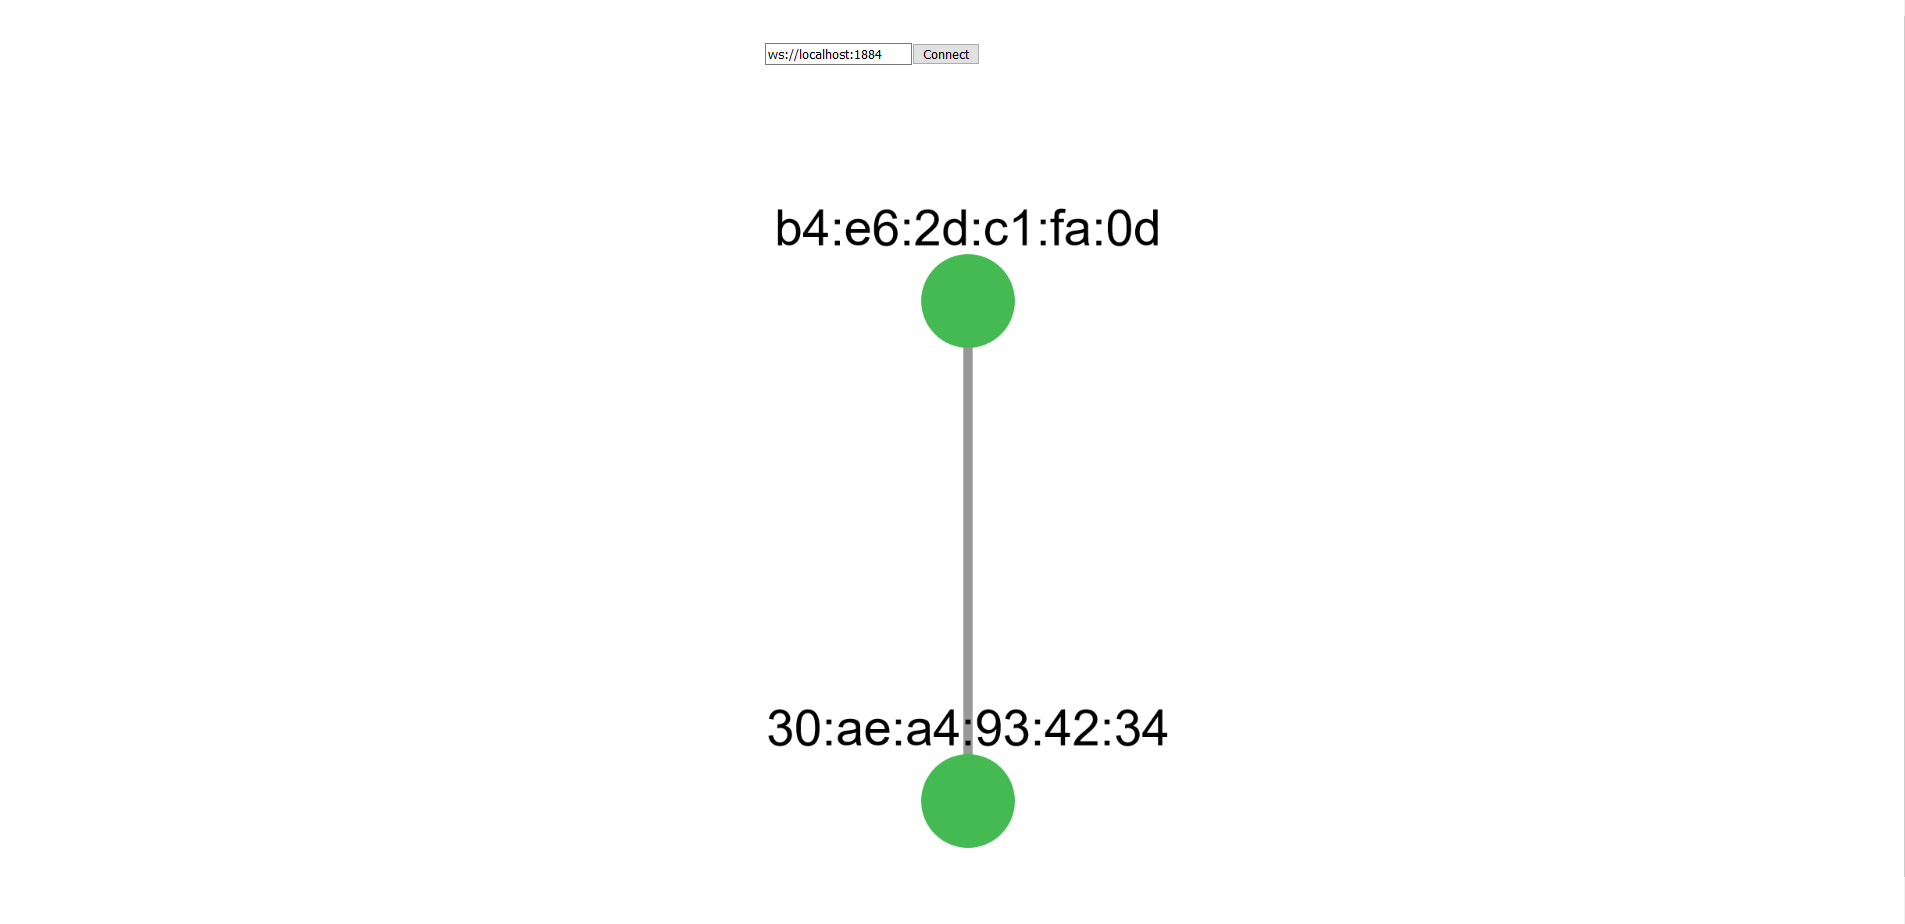
\includegraphics[scale=0.3]{images/example_result_mesh_visualizer.png}
        \caption{Example Ergebnis Mesh Visualizer (Quelle: eigene Darstellung)}
        \label{abb:example_result_mesh_visualizer}
    \end{center}
\end{figure}

In Abbildung \ref{abb:example_result_mesh_visualizer} sieht man wie sich die Mesh Visualizer Website verändert hat.

In dieser Abbildung sind zwei Knoten mit jeweils einer MAC Addresse zu sehen.

Die MAC Addressen stehen für den jeweiligen ESP, der zu diesem Netzwerk verbunden ist.

Die Knoten sind in einer baumartigen Struktur abgebildet. Der Knoten an der Spitz des Diagramms ist der \textbf{Root Knoten}

\subsubsection{Mqtt Fx}
% TODO: Display mqtt messages
\subsection{Code}\label{sec:code}
\subsubsection{Struktur}

\begin{figure}[H]
    \begin{center}
        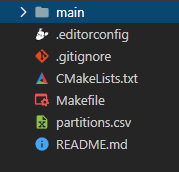
\includegraphics[scale=0.8]{images/example_code_structure_overview.png}
        \caption{Example Code Struktur Übersicht (Quelle: eigene Darstellung)}
        \label{abb:example_code_structure_overview}
    \end{center}
\end{figure}

Die Übersicht in Abbildung \ref{abb:example_code_structure_overview} zeigt einen kleine Ausschnitt der Struktur.

Der Stammordner beinhaltet die Konfigurations Dateien sowie den \textbf{main} Ordner, welcher den Source Code beinhaltet.

Die \textbf{.editorconfig} Datei ist dazu da, die Formatierung des Source Codes in alle Texteditoren uniform zu halten.

In der \textbf{partitions.csv} Datei befindet sich die Beschreibung des in Kapitel \ref{sec:example-partition-table} erwähnten Partition Tables.

Die nachstehende Abbildung zeigt die Struktur des \textbf{main} Ordners.

\begin{figure}[H]
    \begin{center}
        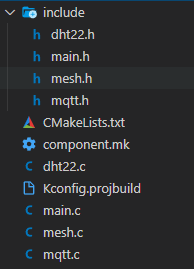
\includegraphics[scale=0.8]{images/example_code_structure_main.png}
        \caption{Example Code Struktur Main (Quelle: eigene Darstellung)}
        \label{abb:example_code_structure_main}
    \end{center}
\end{figure}

Dieser beihnhaltet nicht nur den Source Code sondern auch die \textit{menuconfig} Datei, welche in Kapitel \ref{sec:esp-idf-toolchain} genauer beschrieben ist.

Informationen über die einzelnen Libraries, die im Laufe dieser Arbeit enstanden sind (wie zum Beispiel \textit{mqtt.h}), befinden sich im Kapitel \ref{sec:libraries}.

\subsubsection{Setup}
\subsubsection{IP Event Handler}
\subsubsection{Command Callback}
\subsubsection{DHT22 Task}
\subsection{Mögliche Probleme}
% TODO: Write about possible problems that could occur while following the example

\section{ELF vs. Bin}

\subsection{Bin}
Die Dateierweiterung .bin wird am häufigsten mit komprimierten Binärdateien verknüpft. Diese Dateien werden von vielen verschiedenen Computeranwendungen und für eine Vielzahl von Zwecken verwendet. Die Erweiterung .bin wird häufig für CD- und DVD-Backup-Image-Dateien verwendet.

In einigen Fällen werden die BIN-Dateien im einfachen Binärformat gespeichert und können mit einem Texteditor geöffnet werden. Es gibt jedoch einige BIN-Dateien, die von bestimmten Computeranwendungen erstellt werden und mit der Software geöffnet werden müssen, mit der sie erstellt wurden, oder mit einer kompatiblen Softwareanwendung.\cite{file.org_bin}

\subsection{Hintergrund}
Grundsätzlich sind Binärdateien als solche daran erkennbar, dass der Dateiinhalt, mit einem üblichen Texteditor angezeigt, keine oder überwiegend keine lesbaren Zeichen enthält. Der Versuch, eine Binärdatei als Textdatei zu interpretieren (beispielsweise durch Öffnen mit einem Texteditor), ergibt dann unleserlichen bzw. unsinnigen Text. Für die meisten der heute verwendeten 8-Bit-Zeichensätze gilt: nicht lesbare Steuerzeichen umfassen Zeichen mit ASCII-Werten von 0 bis 31, lesbare Zeichen die mit Werten von 32 bis 126. Die Lesbarkeit von Zeichen mit Werten ab 127 ist abhängig vom verwendeten Zeichensatz. Textdateien können auch gewisse Steuerzeichen enthalten, ohne dass sie deshalb als Binärdatei gelten; dazu gehören Steuerzeichen für Zeilenvorschub, Wagenrücklauf, Seitenumbruch (Seitenvorschub) und Tabulatorzeichen.

Weil Binärdateien alle möglichen Bit-Kombinationen nutzen, bieten sie eine höhere Informationsdichte als Textdateien. Deshalb benötigen sie meist weniger Speicherplatz auf Massenspeichern und lassen sich schneller laden und speichern. Ferner lassen sich darin verschiedene Objekttypen (beispielsweise Text mit Bildern) relativ einfach ablegen.

Binärformate werden beim Austausch über verschiedene Plattformen hinweg (beispielsweise Windows, Macintosh, Linux) nicht beschädigt, da die jeweiligen Softwarekomponenten nicht versuchen, die Dateien für die Zielplattform zu konvertieren. Andererseits wird der systemübergreifende Datenaustausch erschwert, da Binärdateien häufig Daten in einem systemabhängigen Format enthalten. (Beispielsweise Zahlen im Big- oder Little-Endian-Format.) Die Spezifikation des Dateiformats einer Binärdatei legt fest, wie mit der Datei zu verfahren ist. Zum Lesen, Bearbeiten und Speichern binärer Datenformate benötigt man im Allgemeinen spezielle, auf das Dateiformat abgestimmte Editoren (beispielsweise Textverarbeitung für Office-Texte, ein Bildbearbeitungsprogramm für Fotos, regedit für die Windows-Registrierungsdatenbank).

Zu beachten ist, dass man unter einer Binärdatei bzw. unter Binärformat nicht Daten versteht, die nur aus den (sichtbaren) Zeichen „0“ und „1“ aufgebaut sind – wie die Namensanalogie zu Hex(adezimal)datei nahelegen könnte. Binärdatei bedeutet auch nicht, dass die Daten nur aus binären „0“ und „1“ bestehen – weil das auch bei Text-Zeichensätzen der Fall ist. Auch ist eine Datei, die von einem Textverarbeitungsprogramm erzeugt wurde, meist (abhängig vom Dateiformat) keine reine Textdatei im engeren Sinn, sondern eine Binärdatei, in der zum Beispiel Formatangaben und andere Steuerzeichen nicht mit einem lesbaren Zeichensatz codiert sind. Solche Dateien, zum Beispiel im Rich-Text-Format, sind insofern eine Mischform aus Text- und Binärdatei.\cite{bin_wikipedia}

\subsection{ELF}
ELF ist die Abkürzung für Executable and Linkable Format und definiert die Struktur für Binärdateien, Bibliotheken und Core-Dateien. Die formale Spezifikation ermöglicht es dem Betriebssystem, die zugrunde liegenden Maschinenanweisungen korrekt zu interpretieren. ELF-Dateien sind normalerweise die Ausgabe eines Compilers oder Linkers und haben ein Binärformat.
\newline
\newline
Ein häufiges Missverständnis ist, dass ELF-Dateien nur für Binärdateien oder ausführbare Dateien bestimmt sind. Es ist jedoch möglich sie für Teilstücke (Objektcode) verwendet zu können. Ein weiteres Beispiel sind gemeinsam genutzte Bibliotheken oder sogar Core-Dumps (Core- oder a.out-Dateien). Die ELF-Spezifikation wird auch unter Linux für den Kernel selbst und die Linux-Kernelmodule verwendet.


\subsection{Struktur}
Aufgrund des erweiterbaren Designs von ELF-Dateien unterscheidet sich die Struktur je nach Datei. Eine ELF-Datei besteht aus:

\begin{itemize} 
\item ELF-Header
\item Dateidaten
\end{itemize}

Mit dem Befehl readelf können wir uns die Struktur einer Datei ansehen und sie sieht ungefähr so aus:

\begin{figure}[H]
    \begin{center}
        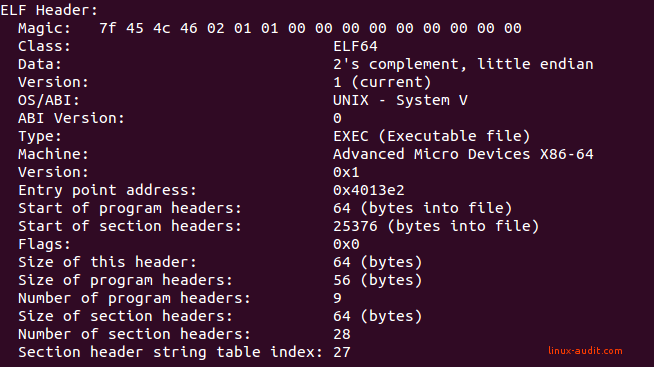
\includegraphics[scale=0.5]{images/elf-header-linux-binary.png}
        \caption{Details einer Elf-binary \cite{details_of_Elf_binary}}
    \end{center}
\end{figure}
 
\subsection{ELF-Header}
Wie in diesem Screenshot zu sehen ist, beginnt der ELF-Header mit etwas Magic. Diese ELF-Header-Magic liefert Informationen über die Datei. Die ersten 4 hexadezimalen Teile definieren, dass dies eine ELF-Datei ist (45 = E, 4c = L, 46 = F), der der Wert 7f vorangestellt ist.
 
Dieser ELF-Header ist obligatorisch. Es stellt sicher, dass Daten während der Verknüpfung oder Ausführung korrekt interpretiert werden. Um die innere Funktionsweise einer ELF-Datei besser zu verstehen, ist es hilfreich zu wissen, dass diese Header-Informationen verwendet werden.
 
\subsubsection{Class}
Nach der ELF-Typdeklaration ist ein Class-feld definiert. Dieser Wert bestimmt die Architektur für die Datei. Es kann sich um eine 32-Bit- (= 01) oder 64-Bit- (= 02) Architektur handeln. Magic zeigt eine 02, die vom Befehl readelf als ELF64-Datei übersetzt wird. Mit anderen Worten, eine ELF-Datei, die die 64-Bit-Architektur verwendet.

\subsubsection{Data}
Der nächste Teil ist das Data-feld. Es kennt zwei Optionen: 01 für LSB (Least Significant Bit), auch als Little-Endian bekannt. Dann gibt es den Wert 02 für MSB (Most Significant Bit, Big-Endian). Dieser spezielle Wert hilft dabei, die verbleibenden Objekte in der Datei korrekt zu interpretieren. Dies ist wichtig, da verschiedene Prozessortypen unterschiedlich mit den eingehenden Anweisungen und Datenstrukturen umgehen. In diesem Fall wird LSB verwendet, was für Prozessoren vom Typ AMD64 üblich ist.

\subsubsection{Version}
Als nächstes folgt eine weitere "01" in der Magic, die die Versionsnummer ist. Derzeit gibt es nur einen Versionstyp: Derzeit ist dies der Wert "01". Also nichts Interessantes zu merken.

\subsubsection{OS / ABI}
Jedes Betriebssystem hat eine große Überlappung in gemeinsamen Funktionen. Darüber hinaus hat jedes von ihnen spezifische oder zumindest geringfügige Unterschiede. Die Definition des richtigen Sets erfolgt über eine Application Binary Interface (ABI). Auf diese Weise wissen sowohl das Betriebssystem als auch die Anwendungen, was zu erwarten ist, und die Funktionen werden korrekt weitergeleitet. Diese beiden Felder beschreiben, für was ABI verwendet wird und die zugehörige Version. In diesem Fall ist der Wert 00, was bedeutet, dass keine bestimmte Erweiterung verwendet wird. Die Ausgabe zeigt dies als System V.

\subsubsection{ABI-Version}
Bei Bedarf kann eine Version für das ABI angegeben werden.

\subsubsection{Machine}
Den Maschinentyp (AMD64) finden wir auch im Header.

\subsubsection{Type}
Das Typfeld gibt an, wozu die Datei dient. Es gibt einige gängige Dateitypen.

\begin{itemize}
\item CORE (Wert 4)
\item DYN (Shared Object File) für Bibliotheken (Wert 3)
\item EXEC (ausführbare Datei) für Binärdateien (Wert 2)
\item REL (verschiebbare Datei), bevor sie in eine ausführbare Datei gelinked wird (Wert 1)
\end{itemize}

\subsection{File Data}
Neben dem ELF-Header bestehen ELF-Dateien aus drei Teilen.

\begin{itemize}
\item Program Headers oder Segments (9)
\item Section Headers oder Sections (28)
\item Data
\end{itemize}

Außerdem ist es gut zu wissen, dass ELF zwei sich ergänzende „Ansichten“ hat. Eine Benutzeroberfläche muss für den Linker verwendet werden, um die Ausführung zu ermöglichen (segments). Die andere zum Kategorisieren von Anweisungen und Daten (sections). Je nach Ziel werden also die zugehörigen Headertypen verwendet.

\subsubsection{Programm-Header}
Eine ELF-Datei besteht aus null oder mehr Segmenten und beschreibt, wie ein process/memory image für die Laufzeitausführung erstellt wird. Wenn der Kernel diese Segmente sieht, verwendet er sie, um sie mithilfe des Systemaufrufs mmap (2) dem virtuellen Adressraum zuzuordnen. Mit anderen Worten, es konvertiert vordefinierte Anweisungen in ein Speicherbild. Wenn Ihre ELF-Datei eine normale Binärdatei ist, sind diese Programmheader erforderlich. Andernfalls wird es einfach nicht ausgeführt. Diese Header mit der zugrunde liegenden Datenstruktur werden verwendet, um einen Prozess zu bilden. Dieser Vorgang ist für shared libraries ähnlich.

\begin{figure}[H]
    \begin{center}
        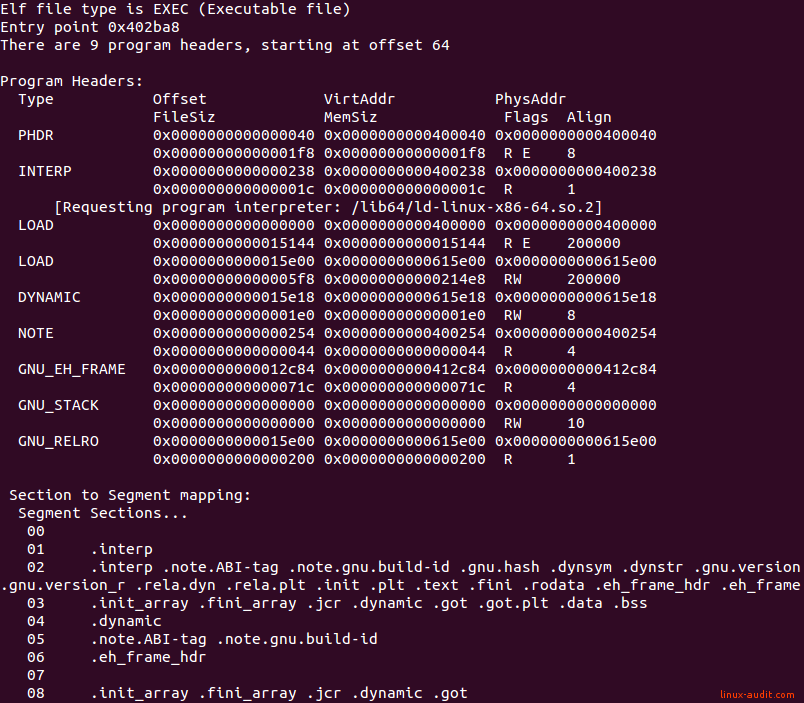
\includegraphics[scale=0.5]{images/elf-program-headers-segments.png}
        \caption{Programm Header einer Elf binary \cite{program_headers_of_Elf_binary}}
    \end{center}
\end{figure}

\subsubsection{GNU\_EH\_FRAME}
Dies ist eine sorted queue, die vom GNU C-Compiler (gcc) verwendet wird. Es speichert Ausnahmebehandlungsroutinen. Wenn also etwas schief geht, kann es diesen Bereich verwenden, um richtig damit umzugehen.

\subsubsection{GNU\_STACK}
Dieser Header wird zum Speichern von stack-Informationen verwendet. Der stack ist ein Puffer oder eine Arbeitsstelle, an der Elemente wie lokale Variablen gespeichert werden. Dies geschieht bei LIFO (Last In, First Out). Beim Starten einer Prozessfunktion wird ein Baustein reserviert. Wenn die Funktion beendet ist, wird sie wieder als frei markiert. Der interessante Teil ist nun, dass ein Stack nicht ausführbar sein sollte, da dies zu Sicherheitslücken führen kann. Durch Manipulation des Speichers könnte man auf diesen ausführbaren stack verweisen und beabsichtigte Anweisungen ausführen.

Wenn das Segment GNU\_STACK nicht verfügbar ist, wird normalerweise ein executable stack verwendet.
Die Tools scanelf und execstack sind zwei Beispiele, um die stack-Details anzuzeigen.

\begin{figure}[H]
    \begin{center}
        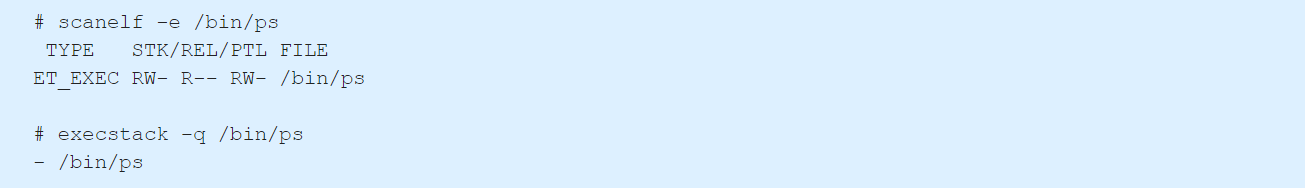
\includegraphics[scale=1]{images/example_gnustack.png}
        \caption{Beispiel GNU\_STACK \cite{example_gnustack}}
    \end{center}
\end{figure}

\subsection{Static vs. Daynamic binaries}
Beim Umgang mit ELF-Binärdateien ist es gut zu wissen, dass es zwei Typen gibt und wie sie verknüpft sind. Der Typ ist entweder statisch oder dynamisch und bezieht sich auf die verwendeten Bibliotheken. Zu Optimierungszwecken stellen wir häufig fest, dass Binärdateien „dynamisch“ sind, was bedeutet, dass externe Komponenten für die ordnungsgemäße Ausführung erforderlich sind. Häufig handelt es sich bei diesen externen Komponenten um normale Bibliotheken, die allgemeine Funktionen wie das Öffnen von Dateien oder das Erstellen eines Netzwerk-Sockets enthalten. In statischen Binärdateien sind dagegen alle Bibliotheken enthalten. Dadurch werden sie größer und dennoch tragbarer (z. B. wenn sie auf einem anderen System verwendet werden).

\subsection{Fazit}
ELF-Dateien dienen zur Ausführung oder zum Verknüpfen. Abhängig vom primären Ziel enthält es die erforderlichen Segmente oder Abschnitte. Segmente werden vom Kernel angeschaut und auf den Speicher gemappt (mithilfe von mmap). Abschnitte werden vom Linker angeschaut, um ausführbaren Code oder freigegebene Objekte zu erstellen.

Der ELF-Dateityp ist sehr flexibel und bietet Unterstützung für mehrere CPU-Typen, Maschinenarchitekturen und Betriebssysteme. Es ist auch sehr erweiterbar: Jede Datei ist je nach den erforderlichen Teilen unterschiedlich aufgebaut.

Header bilden einen wichtigen Teil der Datei und beschreiben genau den Inhalt einer ELF-Datei. Mit den richtigen Tools erhalten Sie ein grundlegendes Verständnis des Zwecks der Datei. Von dort aus können Sie die Binärdateien weiter überprüfen. Dies kann durch Bestimmen der zugehörigen Funktionen oder der in der Datei gespeicherten Zeichenfolgen erfolgen.\cite{elf_linux_audit}